\chapter{Complex Manifolds}

In this chapter we introduce the elements of several complex variables and the notion of complex manifolds.
We also provide some examples of complex ma\-nifolds.

\section{Holomorphic maps}

\begin{defn}
    A complex valued function $f(z)$ on a connected open subset $W\subset\mathbb{C}^n$ is called \emph{holomorphic}, if for each $a=(a_1,\cdots,a_n)\in W$, $f(z)$ can be expanded as a convergent power series
    \[f(z)=\sum_{k_1\geq 0,\cdots,k_n\geq 0}c_{k_1\cdots k_n}(z_1-a_1)^{k_1}\cdots(z_n-a_n)^{k_n}\]
    in some neighborhood of $a$.
\end{defn}

From now on we shall use \emph{domain} to denote a connected open set.

\begin{prop}
    If $p(z)=\sum c_{k_1\cdots k_n}(z_1-a_1)^{k_1}\cdots(z_n-a_n)^{k_n}$ converges at $z=w$, then $p(z)$ converges for every $z$ with $|z_k-a_k|<|w_k-a_k|,\ k=1,\cdots,n$.
\end{prop}
\begin{proof}
    Left to reader.
\end{proof}

\begin{defn}
    The neighborhood above is called a \emph{polydisc} or \emph{polycylinder}, and denoted by 
    \[P(a,r)=\{z\in\mathbb{C}^n:\ |z_k-a_k|<r_k,\ k=1,2,\cdots,n\}\]
\end{defn}

A complex valued function of $n$ complex variables can be seen as a function of $2n$ real variables, thus we have the following definition.
\begin{defn}
    A complex valued function of $n$ complex variables is \emph{continuous} or \emph{differentiable}, if it is continuous or differentiable as a function of $2n$ real variables.
\end{defn}

We have

\begin{thm}[Osgood]\label{osgood}
    Let $f(z_1,\cdots,z_n)$ be a continuous function on the domain $W\subset\mathbb{C}^n$, if $f$ is holomorphic with respected to each $z_k$ and other $z_i$'s fixed, then $f$ is holomorphic on $W$.
\end{thm}
\begin{proof}
    Let $a\in W$ lie in the polydisc $\overline{P(a,r)}\subset W$.
    For $z\in P(a,r)$, we use Cauchy's integral formula iteratively:
    \begin{gather*}
        f(z_1,z_2,\cdots,z_n)=\frac{1}{2\pi\sqrt{-1}}\int_{|w_1-a_1|=r_1}\frac{f(w_1,z_2,\cdots,z_n)}{w_1-z_1}\d{w_1}\\
        f(w_1,z_2,\cdots,z_n)=\frac{1}{2\pi\sqrt{-1}}\int_{|w_2-a_2|=r_2}\frac{f(w_1,w_2,\cdots,z_n)}{w_2-z_2}\d{w_2}\\
        \cdots
    \end{gather*}
    Substituting, we have
    \[\left(\frac{1}{2\pi\sqrt{-1}}\right)^n\idotsint_{\partial P(a,r)}\frac{f(w_1,\cdots,w_n)}{(w_1-z_1)\cdots(w_n-z_n)}\d{w_1}\cdots\d{w_n}\]
    Since
    \[\left|\frac{z_k-a_k}{w_k-a_k}\right|<1\]
    The series
    \begin{align*}
        \frac{1}{w_k-z_k}&=\frac{1}{(w_k-a_k)-(z_k-a_k)}=\frac{1}{w_k-a_k}\cdot\frac{1}{1-(z_k-a_k)/(w_k-a_k)}\\
        &=\frac{1}{w_k-a_k}\sum_{i=0}^\infty\left(\frac{z_k-a_k}{w_k-a_k}\right)^i
    \end{align*}
    converges absolutely in $P(a,r)$, hence integrate term by term we have
    \[f(z_1,\cdots,z_n)=\sum_{k_0\geq 0,\cdots,k_n\geq 0}c_{k_1\cdots k_n}(z_1-a_1)^{k_1}\cdots(z_n-a_n)^{k_n}\]
    where
    \[c_{k_1\cdots k_n}=\left(\frac{1}{2\pi\sqrt{-1}}\right)^{k_1+\cdots+k_n}\idotsint_{\partial P(a,r)}\frac{f(w_1,\cdots,w_n)\d{w_1}\cdots\d{w_n}}{(w_1-a_1)^{k_1+1}\cdots(w_n-a_n)^{k_n+1}}\]
    Let $|f|\leq M$ on $\overline{P(a,r)}$, then we have
    \[|c_{k_0\cdots k_n}|\leq\frac{M}{r_1^{k_1}\cdots r_n^{k_n}}\]
    and for $z\in P(a,r)$, we have $|(z_k-a_k)/r_k|<1$, then
    \begin{align*}
        \left|\sum c_{k_1\cdots k_n}(z_1-a_1)^{k_1}\cdots(z_n-a_n)^{k_n}\right|&\leq M\left|\sum\left(\frac{z_1-a_1}{r_1}\right)^{k_1}\cdots\left(\frac{z_n-a_n}{r_n}\right)^{k_n}\right|\\
        &=M\prod_{k=1}^n\left|\frac{1}{1-(z_k-a_k)/r_k}\right|
    \end{align*}
    This shows the expansion is convergent for $z\in P(a,r)$.
    Since $a$ is arbitrary, $f$ is holomorphic.
\end{proof}

We now introduce the Cauchy--Riemann equations.

\begin{sym}
    Let $f$ be a differentiable function on a domain $W\subset\mathbb{C}^n$, denote
    \begin{gather}
        \frac{\partial}{\partial z_k}=\frac{1}{2}\left(\frac{\partial}{\partial x_k}-\sqrt{-1}\frac{\partial}{\partial y_k}\right)\\
        \frac{\partial}{\partial\overline{z_k}}=\frac{1}{2}\left(\frac{\partial}{\partial x_k}+\sqrt{-1}\frac{\partial}{\partial y_k}\right)
    \end{gather}
    for $z_k=x_k+\sqrt{-1}y_k$ and $1\leq k\leq n$.
\end{sym}

\begin{thm}
    Let $f$ be a (continuously) differentiable function on the domain $W\subset\mathbb{C}^n$, then $f$ is holomorphic on $W$ if and only if $\partial{f}/\partial{\overline{z_k}}=0$ for $k=1,\cdots,n$.
\end{thm}
\begin{proof}
    This is a corollary of Theorem~\ref{osgood} and classical results in complex analysis in one variable.
\end{proof}

\begin{prop}[Chain rule]
    Suppose $f(w_1,\cdots,w_m)$ and $g_k(z),\ k=1,\cdots,m$ are differentiable, and the domain of $f$ contains the range of $g=(g_1,\cdots,g_m)$, then $f\circ g$ is differentiable, and if $w_i=g_i(z)$ for $i=1,\cdots,m$, then
    \begin{gather*}
        \frac{\partial f(g(z)))}{\partial z_k}=\sum_{i=1}^m\left(\frac{\partial f(w)}{\partial w_i}\cdot\frac{\partial w_i}{\partial z_k}+\frac{\partial f(w)}{\partial\overline{w_i}}\cdot\frac{\partial\overline{w_i}}{\partial z_k}\right)\\
        \frac{\partial f(g(z)))}{\partial\overline{z_k}}=\sum_{i=1}^m\left(\frac{\partial f(w)}{\partial w_i}\cdot\frac{\partial w_i}{\partial\overline{z_k}}+\frac{\partial f(w)}{\partial\overline{w_i}}\cdot\frac{\partial\overline{w_i}}{\partial\overline{z_k}}\right)
    \end{gather*}
\end{prop}
\begin{proof}
    Direct calculation verifies the proposition.
\end{proof}

\begin{cor}
    If $f(w)$ is holomorphic in $w=(w_1,\cdots,w_m)$ and $g_k(z),\ k=1,\cdots,m$ are holomorphic in $z$, then $f\circ g$ is holomorphic in $z$.
\end{cor}

\begin{cor}
    The set $\mathcal{O}_{\mathbb{C}^n}(\Omega)$ of holomorphic functions on open set $\Omega$ forms a ring. (We use sheaf notation before we introduce what is a sheaf.)
\end{cor}

\begin{defn}
    A map $f(z)=(f_1(z),\cdots,f_m(z))$ from $\mathbb{C}^n$ to $\mathbb{C}^m$ is a \emph{holomorphic map} if each $f_k(z)$ is holomorphic, $k=1,\cdots,m$.
    The matrix
    \[\begin{bmatrix}
        \partial{f_1}/\partial{z_1} & \cdots & \partial{f_m}/\partial{z_1}\\
        \vdots & \ddots & \vdots \\
        \partial{f_1}/\partial{z_n} & \cdots & \partial{f_m}/\partial{z_n}
    \end{bmatrix}=:\left[\frac{\partial{f_i}}{\partial{z_j}}\right]_{1\leq i\leq m,1\leq j\leq n}\]
    is called \emph{Jacobian matrix}, and if $m=n$, the determinant $\det[\partial{f_i}/\partial{z_j}]$ is called the \emph{Jacobian}.
\end{defn}

Writing out $f_i=u_i+\sqrt{-1}v_i$ and $z_j=x_j+\sqrt{-1}y_j$, we denote briefly
\[\frac{\partial(u,v)}{\partial(x,y)}:=\det\left(\frac{\partial(u_1,v_1,\cdots,u_n,v_n)}{\partial(x_1,y_1,\cdots,x_n,y_n)}\right)\]
And we have
\begin{lem}\label{real jacobian}
    If $f$ is holomorphic, then $\partial(u,v)/\partial(x,y)=|\det[\partial{f_i}/\partial{z_j}]|^2\geq 0$.
\end{lem}
\begin{proof}
    Let
    \begin{gather*}
        \begin{bmatrix}
            \partial/\partial{z_1} & \partial/\partial{\overline{z_1}} & \cdots & \partial/\partial{z_n} & \partial/\partial{\overline{z_n}}
        \end{bmatrix}=A\\
        \begin{bmatrix}
            \partial/\partial{x_1} & \partial/\partial{y_1} & \cdots & \partial/\partial{x_n} & \partial/\partial{y_n}
        \end{bmatrix}=B
    \end{gather*}
    Then
    \[A=B\begin{bmatrix}
        1/2 & 1/2 & & & \\
        -\sqrt{-1}/2 & \sqrt{-1}/2 & & & \\
         & & 1/2 & 1/2 & \\
         & & -\sqrt{-1}/2 & \sqrt{-1}/2 & \\
         & & & & \ddots
    \end{bmatrix}\]
    Hence
    \begin{align*}
        \frac{\partial(u,v)}{\partial(x,y)}&=\det\begin{bmatrix}
            u_1 \\ v_1 \\ \vdots \\ u_n \\ v_n
        \end{bmatrix}\begin{bmatrix}
            \partial/\partial{x_1} & \partial/\partial{y_1} & \cdots & \partial/\partial{x_n} & \partial/\partial{y_n}
        \end{bmatrix}\\
        &=\left(\frac{\sqrt{-1}}{2}\right)^n\det\begin{bmatrix}
            u_1 \\ v_1 \\ \vdots \\ u_n \\ v_n
        \end{bmatrix}\begin{bmatrix}
            \partial/\partial{z_1} & \partial/\partial{\overline{z_1}} & \cdots & \partial/\partial{z_n} & \partial/\partial{\overline{z_n}}
        \end{bmatrix}\\
        &=\left(\frac{\sqrt{-1}}{2}\right)^n\det\begin{bmatrix}
            \partial{u_1}/\partial{z_1} & \partial{u_1}/\partial{\overline{z_1}} & \cdots & \partial{u_1}/\partial{z_n} & \partial{u_1}/\partial{\overline{z_n}}\\
            \partial{v_1}/\partial{z_1} & \partial{v_1}/\partial{\overline{z_1}} & \cdots & \partial{v_1}/\partial{z_n} & \partial{v_1}/\partial{\overline{z_n}}\\
            \vdots & \vdots & \ddots & \vdots & \vdots \\
            \partial{u_n}/\partial{z_1} & \partial{u_n}/\partial{\overline{z_1}} & \cdots & \partial{u_n}/\partial{z_n} & \partial{u_n}/\partial{\overline{z_n}}\\
            \partial{v_n}/\partial{z_1} & \partial{v_n}/\partial{\overline{z_1}} & \cdots & \partial{v_n}/\partial{z_n} & \partial{v_n}/\partial{\overline{z_n}}
        \end{bmatrix}
    \end{align*}
    Multiply $\sqrt{-1}$ on even rows, $1/2$ on odd rows, and add $2k$th row to ($2k-1$)st row, subtract ($2k-1$)st row to $2k$th row, we obtain
    \[\frac{\partial(u,v)}{\partial(x,y)}=\det\begin{bmatrix}
        \partial{f_1}/\partial{z_1} & & \cdots & \partial{f_1}/\partial{z_n} & \\
         & \overline{\partial{f_1}/\partial{z_1}} & \cdots & & \overline{\partial{f_1}/\partial{z_n}} \\
        \vdots & \vdots & \ddots & \vdots & \vdots \\
        \partial{f_n}/\partial{z_1} & & \cdots & \partial{f_n}/\partial{z_n} & \\
        & \overline{\partial{f_n}/\partial{z_1}} & \cdots & & \overline{\partial{f_n}/\partial{z_n}}
    \end{bmatrix}\]
    We expand the determinant, extract odd rows and even rows respectively, and we get
    \begin{align*}
        \frac{\partial(u,v)}{\partial(x,y)}&=\sum_{\sigma,\tau\in S_n}\sgn\sigma\sgn\tau\left(\frac{\partial{f_1}}{\partial{z_{\sigma(1)}}}\cdots\frac{\partial{f_n}}{\partial{z_{\sigma(n)}}}\right)\left(\overline{\frac{\partial{f_1}}{\partial{z_{\tau(1)}}}}\cdots\overline{\frac{\partial{f_n}}{\partial{z_{\tau(n)}}}}\right)\\
        &=\det[\partial{f_i}/\partial{z_j}]\overline{\det[\partial{f_i}/\partial{z_j}]}\\
        &=|\det[\partial{f_i}/\partial{z_j}]|^2\qedhere
    \end{align*}
\end{proof}

\begin{thm}[Inverse function theorem]
    Let $U\subset\mathbb{C}^n$ open, $f:U\to\mathbb{C}^n$ be a holomorphic map, $a\in U$.
    If $\det[\partial{f_i}/\partial{z_j}]_{z=a}\neq 0$, then for a sufficiently small neighborhood $N$ of $a$, $f$ is bijective on $N$, $f(N)$ is open and $f^{-1}|_{f(N)}$ is holomorphic on $f(N)$.
\end{thm}
\begin{proof}
    By Lemma~\ref{real jacobian}, $\partial(u,v)/\partial(x,y)\neq 0$ at $a$, then by the inverse function theorem of real functions, $f$ is bijective and differentiable, and $f(N)$ is open.
    We check that $f^{-1}|_{f(N)}$ is holomorphic.
    Set $\varphi(w)=f^{-1}(w)$, then $z_i=\varphi_i(f(z))$.
    Differentiate the equality gives
    \begin{align*}
        0=\frac{\partial z_i}{\partial\overline{z_k}}&=\sum_{j=1}^n\left(\frac{\partial\varphi_i(w)}{\partial w_j}\cdot\frac{\partial f_j(z)}{\partial\overline{z_k}}+\frac{\partial\varphi_i(w)}{\partial\overline{w_j}}\cdot\frac{\partial\overline{f_j(z)}}{\partial\overline{z_k}}\right)\\
        &=\sum_{j=1}^n\frac{\partial\varphi_i(w)}{\partial\overline{w_j}}\cdot\frac{\partial\overline{f_j(z)}}{\partial\overline{z_k}}
    \end{align*}
    Since $\det[\partial\overline{f_j(z)}/\partial\overline{z_k}]=\overline{\det[\partial f_j(z)/z_k]}\neq 0$, by linear algebra we have $\partial\varphi_i(w)/\partial\overline{w_j}=0$ for each $i,j$, that is, $\varphi$ is holomorphic.
\end{proof}

\begin{cor}[Implicit function theorem]
    Let $f_i$, $i=1,2,\cdots,m$ be holomorphic on $U\subset\mathbb{C}^n$.
    Let rank of $[\partial f_i/\partial z_j]=r$ at each point $z\in U$ and suppose $\det[\partial f_i/\partial z_j]_{1\leq i,j\leq r}\neq 0$.
    If $f_i(a)=0$ for $i\leq m$ for some $a\in U$, then in a small neighborhood of $a$, the equations
    \[f_i(z_1,\cdots,z_r,z_{r+1},\cdots,z_n)=0,\quad 1\leq i\leq r\]
    have unique holomorphic solutions
    \[z_i=\varphi_i(z_{r+1},\cdots,z_n),\quad 1\leq i\leq r\]
\end{cor}

\section{Complex Manifolds}

\begin{defn}
    Let $M$ be a topological manifold.
    A \emph{coordinate chart} is an open set $U\subset M$ and a continuous map $\varphi:U\to\mathbb{C}^n$ that maps $U$ homeomorphically onto an open set of $\mathbb{C}^n$.
    An \emph{atlas} is a collection $\{(U_i,\varphi_i)\}_{i\in I}$ of coordinate charts that $M=\bigcup_{i\in I}U_i$ and for any $U_i\cap U_j\neq\varnothing$, $\varphi_i\circ\varphi_j^{-1}$ and $\varphi_j\circ\varphi_i^{-1}$ are both holomorphic.
    A \emph{complex structure} is a maximal atlas.

    A \emph{complex manifold} is a topological manifolds endowed with a complex structure.
\end{defn}

\begin{lem}
    Every complex manifold is paracompact, i.e.\ every open cover has a locally finite open refinement.
\end{lem}
\begin{proof}
    \cite[Theorem~4.77]{LeeTop}.
\end{proof}

\begin{defn}
    Let $M$ be a complex manifold.
    A subset $S\subset M$ is a (complex) \emph{analytic subvariety}, if for each $s\in S$, there is a neighborhood $U$ of $s$ such that $S\cap U=\{p:\ f_i(p)=0,\ i=1,\cdots,m\}$ for holomorphic functions $f_i,\ i=1,\cdots,m$.
    The analytic subvariety is a \emph{submanifold} if the rank of $[\partial f_i/\partial z_j]$ is independent of $s$.
\end{defn}

\begin{defn}
    A \emph{meromorphic function} $f$ on $M$ is a complex-valued function defined outside of some proper subvariety $S$ of $M$, and such that given $q\in M$, there is a neighborhood $U$ of $q$ and $g,h$ holomorphic on $U$ satisfying $f(p)=g(p)/h(p)$ on $U\backslash S$.
\end{defn}

\begin{eg}
    \begin{enumerate}
        \item Any holomorphic map $f:M\to\mathbb{CP}^1=\mathbb{C}\cup\{\infty\}$ is meromorphic.
        \item In $\mathbb{C}^2$, we have rational functions $f(z_1,z_2)=P(z_1,z_2)/Q(z_1,z_2)$ for $P,Q$ polynomials are meromorphic.
    \end{enumerate}
\end{eg}

In the rest of the section, we provide some examples and constructions of complex manifolds.

\begin{cons}
    The \emph{complex projective space} $\mathbb{P}^n$ is defined as the set of all $1$-dimensional subspaces of $\mathbb{C}^{n+1}$.
    It can be realized as the sphere $\{z\in\mathbb{C}^{n+1}:\ |z|=1\}=\mathbb{S}^{2n+1}$ quotient out $\mathbb{S}^1$, so it is a compact topological space.
    We denote the elements of $\mathbb{P}^n$ by \emph{homogeneous coordinate} $(p_0,p_1,\cdots,p_n)$.
    The complex projective space is a complex manifolds in the following manner:
    We define $U_j=\{p\in\mathbb{P}^n:\ p_j\neq 0\}$, $j=0,1,\cdots,n$, then $\{U_j\}$ is an open cover of $\mathbb{P}^n$.
    Define $z_j(p)=(z_j^0,\cdots,z_j^{j-1},z_j^{j+1},\cdots,z_j^n)$, where $z_j^i=p_i/p_j$, then $z_j$ maps each $U_j$ homeomorphically onto $\mathbb{C}^n$.
    Moreover, we have $f_{jk}=z_j\circ z_k^{-1}$ given by
    \[(x_1,\cdots,x_k,\cdots,x_n)\mapsto\left(\frac{x_1}{x_j},\cdots,\frac{1}{x_j},\cdots,\frac{x_n}{x_j}\right)\]
    is holomorphic, and so is its inverse.
    Therefore $(U_j,z_j)$ gives an atlas of $\mathbb{P}^n$.
\end{cons}

In projective space, we have the notion of algebraic objects.

\begin{defn}
    Let $\mathbb{P}^n$ has homogeneous coordinate $\zeta=(\zeta_0,\cdots,\zeta_n)$.
    A \emph{projective algebraic variety} $M$ is the common zero locus of a family of homogeneous polynomials, i.e.\ for some homogeneous polynomials $f_1,\cdots,f_m$, 
    \[M:=\{\zeta\in\mathbb{P}^n:\ f_i(\zeta)=0,\ i=1,\cdots,m\}\]
    If the the rank of $[\partial{f_i}/\partial{\zeta_j}]$ is independent from $\zeta$, then $M$ becomes a manifold, called \emph{algebraic manifold}.
    Alternatively, we can define algebraic manifolds as submanifolds of projective spaces, by \textsc{Chow}'s theorem (cf.\ \cite[Section~3.3]{Griffiths74}),these two definitions of algebraic manifolds are equivalent.
    If $f_d$ is a homogeneous polynomial of degree $d$, then its zero locus $M_d$ is called a \emph{hypersurface} in $\mathbb{P}^n$ of order $d$.
    If for each $\zeta\in M_d$, at least one of $\partial f_d/\partial\zeta_i\neq 0$, then $M_d$ is nonsingular.
\end{defn}

\begin{eg}
    We provide some examples.
    \begin{enumerate}
        \item $M_d\subset\mathbb{P}^2$ a nonsingular plane curve of order $d$ is a Riemann surface of genus $g=\frac{1}{2}(d-1)(d-2)$. (cf.~\cite[pp.\ 219--221]{G-H})
        \item A nonsingular $M_d\subset\mathbb{P}^3$.
        $M_d$ is simply connected and has Euler number $\chi(M_d)=d(d^2-4d+6)$.
        (For Euler number, cf.~\cite[Section 10.2, Equation (5)]{Hirzebruch95}, and for simply connectivity, cf.~\cite[Theorem 7.4]{Milnor63})
        \item Let $M\subset\mathbb{P}^3$ be defined by
        \[M=\{\zeta\in\mathbb{P}^3:\ \zeta_1\zeta_2-\zeta_0\zeta_3=0,\zeta_0\zeta_2-\zeta_1^2=0,\zeta_2^2-\zeta_1\zeta_3=0\}\]
        We claim that $M$ is complex analytically homeomorphic to $\mathbb{P}^1$.
        One can easily check the map
        \[\mu:\mathbb{P}^1\to\mathbb{P}^3,t\mapsto(t_0^3,t_0^2t_1,t_0t_1^2,t_1^3)\]
        is biholomorphic.
        This is the simplest case of \emph{Veronese embedding}.
    \end{enumerate}
\end{eg}

Next we consider \emph{quotient spaces}.

\begin{defn}
    An \emph{analytic automorphism} of $M$ is a biholomorphic map of $M$ onto $M$.
    The set of all analytic automorphisms of $M$ forms a group under composition.

    Let $G$ be a subgroup of analytic automorphisms.
    $G$ is called a properly \emph{discontinuous group} of analytic automorphisms of $M$, if for any pair of compact subsets $K_1,K_2$, the set $\{g\in G:\ gK_1\cap K_2\neq\varnothing\}$ is finite.

    $G$ has no fixed points if for all $g\in G,g\neq 1$, $g$ has no fixed points.
\end{defn}

\begin{thm}
    If $M$ is a connected complex manifold, $G$ is properly discontinuous and has no fixed point,  then the quotient space $M/G$ is a complex manifold.
\end{thm}
\begin{proof}
    Denote $M/G=M^*$, and the orbit of $p\in M$ by $p^*$.
    We shall show that for all $q\in M$, we can choose a neighborhood $U\ni q$ such that for all $p_1\neq p_2\in U$ we have $p_1^*\neq p_2^*$.
    In fact, we can choose $U$ such that $gU\cap U=\varnothing$ for $g\in G,g\neq 1$.
    $M$ is locally compact, so let $U_1\supset U_2\supset\cdots$ be a base of relatively compact neighborhoods at $q$.
    Then $F_m=\{g\in G:\ gU_m\cap U_m\neq\varnothing\}$ is finite, and $F_1\supset F_2\supset\cdots$.
    If there is a $g\neq 1$ such that $g\in F_m$ for all $m\geq 1$, then $U_m\to \{q\}$ gives $g(q)=q$, contradicting the nonexistence of fixed points.
    Hence the requiring $U$ exists.
    We cover $M$ by such $U$'s, and $U\to U^*$ is one-to-one.
    We give $U^*$ the complex structure that $U$ has, then this gives a complex structure on $M^*$.
\end{proof}

\begin{eg}[Complex tori]
    Let $M=\mathbb{C}^n$, $\omega_1,\cdots,\omega_{2n}$ be $2n$ $\mathbb{R}$-linear independent vector, $\omega_k=(\omega_{k1},\cdots,\omega_{kn})\in\mathbb{C}^n$.
    Let $G=\mathbb{Z}\omega_1+\cdots+\mathbb{Z}\omega_{2n}$ act on $M$ naturally, then $G$ is properly discontinuous and has no fixed points.
    The quotient space is called \emph{compex torus} of dimension $n$, denoted by $\mathbb{T}^n$.

    Let $n=1$, we have the exponential map $\exp{2\pi\sqrt{-1}}:\mathbb{C}\to\mathbb{C}^*$.
    Consider $G=\mathbb{Z}+\mathbb{Z}\omega$, then $\mathbb{T}=\mathbb{C}/G$.
    But let $\alpha=e^{2\pi\sqrt{-1}\omega}$, for $g=m_1+m_2\omega$, we have the following commutative diagram
    \[\begin{tikzcd}
        \mathbb{C} \ar[r, "\exp{2\pi\sqrt{-1}}"] \ar[d, "g"] &[4mm] \mathbb{C}^* \ar[d, "\alpha^{m_2}"] \\
        \mathbb{C} \ar[r, "\exp{2\pi\sqrt{-1}}"] &[4mm] \mathbb{C}^*
    \end{tikzcd}\]
    Hence if we let $G^*=\mathbb{Z}\omega$ act on $\mathbb{C}^*$ by multiplication, then we have $\mathbb{T}=\mathbb{C}/G=\mathbb{C}^*/G^*$.
\end{eg}

\begin{eg}[Hopf manifolds]
    Let $W=\mathbb{C}^n\setminus\{0\}$ and
    \[G=\{g^m:\ m\in\mathbb{Z},g(w)=\lambda^mw,0<|\lambda|<1\}\]
    It is easy to see $G$ is properly discontinuous and has no fixed points on $W$, so $W/G$ is a complex manifold.
    Moreover, one can show that $W/G$ is diffeomorphic to $\mathbb{S}^1\times\mathbb{S}^{2n-1}$.
    In fact, using polar coordinate we have $W\cong\mathbb{R}_{>0}\times\mathbb{S}^{2n-1}$, scalar multiplication quotients $\mathbb{R}_{>0}$ gets $\mathbb{S}^1$ and preserves $\mathbb{S}^{2n-1}$, hence $W/G\cong\mathbb{S}^1\times\mathbb{S}^{2n-1}$ as differentiable manifolds.
\end{eg}

\begin{eg}
    Let $M$ be a algebraic surface defined by $M=\{\zeta\in\mathbb{P}^3:\ \zeta_0^5+\zeta_1^5+\zeta_2^5+\zeta_3^5=0\}$.
    Let
    \[G=\{g^m:\ g(\zeta_0,\cdots,\zeta_3)=(\rho\zeta_0,\cdots,\rho^4\zeta_3),\rho=e^{2\pi\sqrt{-1}/5}\}\]
    where $m=0,1,2,3,4$.
    Then $g$ is a biholomorphic map $\mathbb{P}^3\to\mathbb{P}^3$ and the restriction of $g^i$ on $M$ is an analytic automorphism.
    Consider the fixed points of $g^m$ on $\mathbb{P}^3$, they satisfy $(\rho^{m(i+1)}-1)\zeta_i=0$, $i=0,1,2,3$.
    So we have the fixed points of $G$ are $(1,0,0,0),(0,1,0,0),(0,0,1,0),(0,0,0,1)$.
    None of the fixed points lies on $M$, so $G$ is properly discontinuous and has no fixed points on $M$, then $M/G$ is a complex manifold.
\end{eg}

Finally we discuss \emph{surgeries}.
Given a complex manifold $M$ and a compact submanifold or subvariety $S\subset M$.
Suppose we have neighborhood $W$ of $S$ and manifolds $S^*\subset W^*$, and we also have a biholomorphic map $f:W^*\setminus S^*\to W\setminus S$.
Then we can replace $W$ by $W^*$ and get a new manifold $M^*=(M\setminus W)\cup W^*$.
More precisely, $M^*=(M\setminus S)\cup W^*$, where each point $z^*\in W^*\setminus S^*$ is identified with $z=f(z^*)$.

\begin{figure}[H]
    \centering
    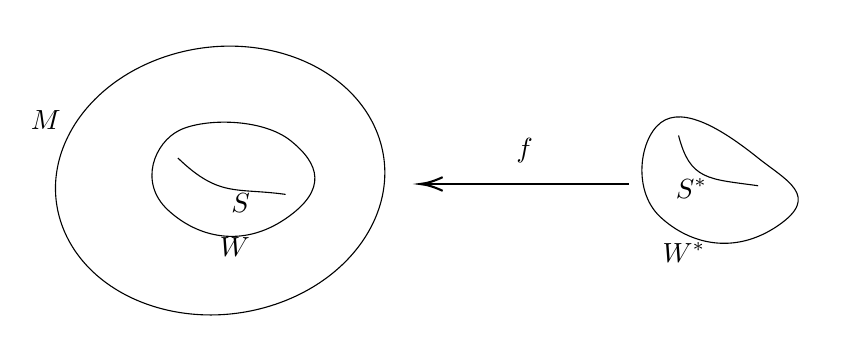
\begin{tikzpicture}[x=0.75pt,y=0.75pt,yscale=-1,xscale=1]
%uncomment if require: \path (0,223); %set diagram left start at 0, and has height of 223

%Shape: Ellipse [id:dp31205351375005885] 
\draw   (35.18,105.18) .. controls (21.37,71.95) and (43.89,34.3) .. (85.46,21.08) .. controls (127.04,7.86) and (171.93,24.08) .. (185.74,57.3) .. controls (199.54,90.53) and (177.03,128.18) .. (135.45,141.4) .. controls (93.87,154.62) and (48.98,138.4) .. (35.18,105.18) -- cycle ;
%Curve Lines [id:da6654336320515477] 
\draw    (90.09,70.38) .. controls (110.06,89.59) and (118.04,84.58) .. (142.01,87.92) ;
%Shape: Polygon Curved [id:ds6403319524310442] 
\draw   (90.89,57.01) .. controls (102.87,51.17) and (130.82,51.17) .. (144.4,62.03) .. controls (157.98,72.89) and (162.77,85.42) .. (142.01,99.62) .. controls (121.24,113.82) and (99.67,108.81) .. (85.3,95.44) .. controls (70.92,82.08) and (78.91,62.86) .. (90.89,57.01) -- cycle ;
%Shape: Polygon Curved [id:ds6985670513888118] 
\draw   (324.92,52) .. controls (336.9,46.15) and (356.07,59.52) .. (369.65,70.38) .. controls (383.23,81.24) and (400,88.76) .. (379.24,102.96) .. controls (358.47,117.16) and (336.9,112.15) .. (322.52,98.78) .. controls (308.15,85.42) and (312.94,57.85) .. (324.92,52) -- cycle ;
%Curve Lines [id:da37504253031609736] 
\draw    (331.31,59.52) .. controls (336.9,81.24) and (345.69,80.4) .. (369.65,83.75) ;
%Straight Lines [id:da1757973560387438] 
\draw    (307.35,82.91) -- (208.71,82.91) ;
\draw [shift={(206.71,82.91)}, rotate = 360] [color={rgb, 255:red, 0; green, 0; blue, 0 }  ][line width=0.75]    (10.93,-3.29) .. controls (6.95,-1.4) and (3.31,-0.3) .. (0,0) .. controls (3.31,0.3) and (6.95,1.4) .. (10.93,3.29)   ;

% Text Node
\draw (109.04,107.33) node [anchor=north west][inner sep=0.75pt]   [align=left] {$\displaystyle W$};
% Text Node
\draw (17.99,46.34) node [anchor=north west][inner sep=0.75pt]   [align=left] {$\displaystyle M$};
% Text Node
\draw (114.54,86.44) node [anchor=north west][inner sep=0.75pt]   [align=left] {$\displaystyle S$};
% Text Node
\draw (322.4,109.67) node [anchor=north west][inner sep=0.75pt]   [align=left] {$\displaystyle W^{*}$};
% Text Node
\draw (328.7,78.76) node [anchor=north west][inner sep=0.75pt]   [align=left] {$\displaystyle S^{*}$};
% Text Node
\draw (251.93,59.71) node [anchor=north west][inner sep=0.75pt]   [align=left] {$\displaystyle f$};


\end{tikzpicture}

    \caption{Surgery}
\end{figure}

\begin{eg}[Hirzebruch]
    Let $M=\mathbb{P}^1\times\mathbb{P}^1$.
    Since $\mathbb{P}^1=\mathbb{C}\cup\{\infty\}$, we can set $S=\{0\}\times\mathbb{P}^1$, $W=\{(z,\zeta)\in\mathbb{C}\times\mathbb{P}^1:\ |z|<\varepsilon\}$ be a neighborhood of $S$ in $M$.
    Let $W^*=\{(z,\zeta)\in\mathbb{C}\times(\mathbb{P}^1)^*:\ |z|<\varepsilon\}$ and $S=\{0\}\times(\mathbb{P}^1)^*$.
    Fix an integer $m>0$ and define $f:W^*\setminus S^*\to W\setminus S$ by
    \[f(z,\zeta^*)=(z,\zeta^*/z^m)\]
    Then $f$ is biholomorphic, let $M_m^*=(M\setminus S)\cup W^*$.
    Hirzebruch proved the following properties in~\cite{Hirzebruch51}:
    \begin{enumerate}
        \item $M$ and $M_m^*$ are topologically different if $m$ is odd.
        \item $M_m^*\not\cong M_n^*$ as complex manifolds when $m\neq n$.
        \item $M^*_{2m}=M$ topologically.
        \item $M^*_{2m+1}=M^*_1$ topologically.
    \end{enumerate}
\end{eg}

\begin{eg}[Blowing up]
    First we discuss the case where $M$ has complex dimension $2$.
    Let $p$ be any point on $M$, $S=\{p\}$ and $S^*=\mathbb{P}^1$.
    We define $M^*=(M\setminus S)\cup\mathbb{P}^1$ as follows:
    Choose a coordinate chart $(W,z)$ such that $z(p)=0$, $|z_1|<\varepsilon,|z_2|<\varepsilon$.
    We define a subvariety $W^*$ of $W\times\mathbb{P}^1$ by
    \[W^*:=\{(z_1,z_2,(\zeta_1,\zeta_2))\in W\times\mathbb{P}^1:\ z_1\zeta_2-z_2\zeta_1=0\}\]
    Since $\partial{f}/\partial{z_1}=\zeta_2,\partial{f}/\partial{z_2}=-\zeta_1$ if $f=z_1\zeta_2-z_2\zeta_1$, $(\partial{f}/\partial{z_1},\partial{f}/\partial{z_2})\neq 0$, hence $W^*$ is a submanifold.
    Let $f^*:W^*\to W$ be the restriction of projection map $W\times\mathbb{P}^1\to W$, then $W^*\supset 0\times\mathbb{P}^1$, $f^*:S^*\to\{p\}$, and $f^*:W^*\setminus S^*\to W\setminus S$ is biholomorphic.
    That is because $f^*$ has inverse $(z_1,z_2)\to(z_1,z_2,(z_1,z_2))$.
    By surgery we obtain $M^*=(M\setminus\{p\})\cup\mathbb{P}^1$.
    We call $M^*$ the \emph{blowing up} of $M$ at $p$, and denote $M^*=\Bl_p(M)$.

    Blowing up can be complicated, a well-known fact in algebraic geometry is for six points $P_1,\cdots,P_6$ in ``general position'' (specified, no three points are colinear and no six points are on a conic), we have
    \[\Bl_{P_6}\cdots\Bl_{P_1}(\mathbb{P}^2)\cong\{\zeta\in\mathbb{P}^3:\ \zeta_0^3+\zeta_1^3+\zeta_2^3+\zeta_3^3=0\}\subset\mathbb{P}^3\]

    General case is similar, if $\dim_\mathbb{C}M=n$, let $p\in M$ and $(W,z)$ be a coordinate chart as above.
    Define the submanifold $W^*:=\{(z,\zeta):\ z_i\zeta_j-z_j\zeta_i=0,\ 1\leq i<j\leq n\}$, and $f^*$ be the restriction of projection map $W\times\mathbb{P}^1\to W$.
    $f^*:(W^*\setminus\mathbb{P}^1)\to(W\setminus\{p\})$ is biholomorphic, so by surgery, we get $\Bl_p(M)=(M\setminus\{p\})\cup\mathbb{P}^1$.
\end{eg}